\section{559 --- Maximum Depth of N-ary Tree}
Given a $n$-ary tree, find its maximum depth.

The maximum depth is the number of nodes along the longest path from the root node down to the farthest leaf node.

For example, given a \texttt{3-ary} tree:

 
\begin{figure}[H]
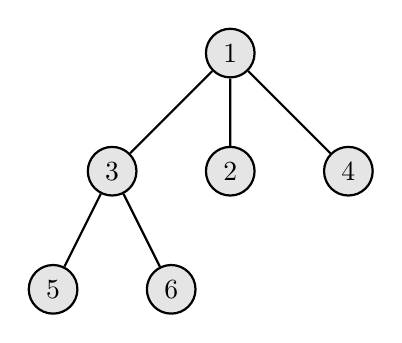
\begin{tikzpicture}
[every node/.style={draw, circle, minimum size=6mm, fill=gray!20!},
  node distance=8mm, 
 thick
]
\node{1}
child{node{3} child{node{5}} child{node{6}}}
child{node{2}}
child{node{4}};
\end{tikzpicture}
\end{figure}

 

We should return its max depth, which is 3.

 

\paragraph{Note:}

\begin{itemize}
\item The depth of the tree is at most 1000.
\item The total number of nodes is at most 5000.
\end{itemize}

\subsection{Recursion}
\begin{itemize}
\item 和计算binary tree的max depth方法类似,对每个child node递归处理,然后结果加上1即为沿着该child node一直往下走的深度。然后所有child node的深度中取最大的深度作为当前node的最大深度。
\end{itemize}

\setcounter{lstlisting}{0}
\begin{lstlisting}[style=customc, caption={Recursion}]
int maxDepth( Node* root )
{
    if( !root )
    {
        return 0;
    }

    int d = 1;

    for( auto node : root->children )
    {
        //1+maxDepth(node) is the depth
        //along with this node
        d = ( max )( d, 1 + maxDepth( node ) );
    }

    return d;
}
\end{lstlisting}